\documentclass[12pt, a4paper]{scrreprt}
\usepackage[margin=2.5cm]{geometry}
\usepackage[hidelinks]{hyperref}
\usepackage{graphicx,xcolor,listings,tikz,enumitem}
\usetikzlibrary{positioning, arrows.meta, shapes, fit}

\definecolor{codegreen}{rgb}{0,0.6,0}
\definecolor{codegray}{rgb}{0.5,0.5,0.5}
\definecolor{codepurple}{rgb}{0.58,0,0.82}
\definecolor{backcolour}{rgb}{0.95,0.95,0.92}

\lstdefinestyle{mystyle}{
  backgroundcolor=\color{backcolour},
  commentstyle=\color{codegreen},
  keywordstyle=\color{blue},
  stringstyle=\color{codepurple},
  basicstyle=\ttfamily\footnotesize,
  numbers=left,
  numbersep=5pt,
  breaklines=true,
  tabsize=2
}
\lstset{style=mystyle}

\newcommand{\faculty}{Faculty Applied Information Technology}
\newcommand{\studies}{Bachelor of Cyber-Security}
\newcommand{\thesistitleDE}{Projekt "WeedDetector" \\ Projektübergabe}
\newcommand{\submissiondate}{05.\ Juli 2025}
\newcommand{\supervisor}{Prof.\ Dr.\ Holger Jehle}

\begin{document}

\begin{titlepage}
  \centering
  {\LARGE Technische Hochschule Deggendorf \\ \faculty \par}
  \vspace{0.3cm}
  {\Large Studiengang \studies \\[1.5cm]}
  {\Huge\bfseries \thesistitleDE\par}
  \vfill
  \begin{minipage}[t]{0.45\textwidth}
    \textbf{Vorgelegt von:}\\
    \\
    Christof Renner (22301943)\\
    Manuel Friedl (1236626)\\
    \\
    \\
    \\
    \\
    Datum: \submissiondate
  \end{minipage}\hfill
  \begin{minipage}[t]{0.45\textwidth}
    \textbf{Prüfungsleitung:}\\
    \\
    \supervisor
  \end{minipage}
\end{titlepage}

\tableofcontents
\newpage

\chapter{Einführung und Projektübersicht}

\section{Motivation und Zielsetzung}
Der \textbf{WeedDetector} ist ein innovatives Softwaresystem, das entwickelt wurde, um in landwirtschaftlichen Umgebungen automatisiert Unkräuter zu erkennen und zu klassifizieren. Die Hauptmotivation hinter diesem Projekt liegt in der zunehmenden Notwendigkeit nachhaltiger landwirtschaftlicher Praktiken und der Reduzierung des Einsatzes von Herbiziden.

Dieses Projekt entstand aus folgenden konkreten Anforderungen:
\begin{itemize}
    \item \textbf{Präzisionslandwirtschaft:} Durch die genaue Identifikation von Unkraut können Landwirte gezielt eingreifen, anstatt flächendeckend Herbizide einzusetzen.
    \item \textbf{Umweltschutz:} Reduzierung des Chemikalieneinsatzes durch punktgenaue Behandlung von Unkrautflächen.
    \item \textbf{Automatisierung:} Integration mit Robotersystemen zur vollautomatischen Unkrautbekämpfung.
    \item \textbf{Kosteneinsparung:} Verringerung des Ressourcenverbrauchs und effizientere Arbeitsabläufe.
\end{itemize}

\section{Systemarchitektur}
Der WeedDetector folgt dem Model-View-Controller (MVC) Architekturmuster, um eine saubere Trennung der Verantwortlichkeiten zu gewährleisten und die Wartbarkeit zu verbessern.

\begin{figure}[h!]
    \centering
    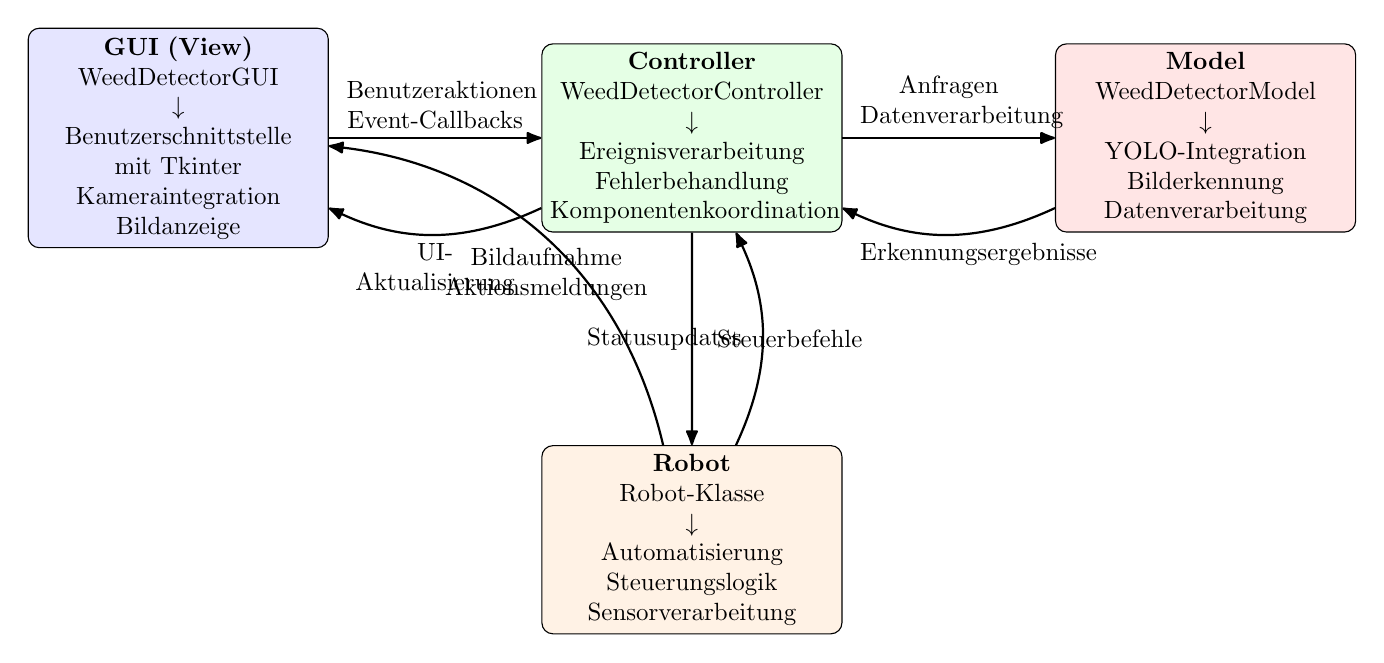
\begin{tikzpicture}[
        scale= 0.9,
        transform shape,
        node distance=3 cm and 3cm,
        box/.style={draw, text width=4cm, align=center, rounded corners, minimum height=2cm},
        arrow/.style={draw, thick, -{Latex[round]}}
    ]

    % Hauptkomponenten
    \node (gui) [box, fill=blue!10] {\textbf{GUI (View)}\\WeedDetectorGUI\\$\downarrow$\\Benutzerschnittstelle mit Tkinter\\Kameraintegration\\Bildanzeige};
    
    \node (controller) [box, right=of gui, fill=green!10] {\textbf{Controller}\\WeedDetectorController\\$\downarrow$\\Ereignisverarbeitung\\Fehlerbehandlung\\Komponentenkoordination};
    
    \node (model) [box, right=of controller, fill=red!10] {\textbf{Model}\\WeedDetectorModel\\$\downarrow$\\YOLO-Integration\\Bilderkennung\\Datenverarbeitung};
    
    \node (robot) [box, below=of controller, fill=orange!10] {\textbf{Robot}\\Robot-Klasse\\$\downarrow$\\Automatisierung\\Steuerungslogik\\Sensorverarbeitung};

    % Verbindungen
    \draw[arrow] (gui) -- node[above, text width=2.5cm, align=center] {Benutzeraktionen\\Event-Callbacks} (controller);
    \draw[arrow] (controller) -- node[above, text width=2.5cm, align=center] {Anfragen\\Datenverarbeitung} (model);
    \draw[arrow] (model) to[bend left=25] node[below, text width=2.5cm, align=center] {Erkennungsergebnisse} (controller);
    \draw[arrow] (controller) to[bend left=25] node[below, text width=2.5cm, align=center] {UI-Aktualisierung} (gui);
    \draw[arrow] (controller) -- node[right, text width=2.5cm, align=center] {Steuerbefehle} (robot);
    \draw[arrow] (robot) to[bend right=25] node[left, text width=2.5cm, align=center] {Statusupdates} (controller);
    \draw[arrow] (robot) to[bend right=35] node[below, text width=3.5cm, align=center] {Bildaufnahme\\Aktionsmeldungen} (gui);

    \end{tikzpicture}
    \caption{Detaillierte Architektur des WeedDetector-Systems}
    \label{fig:systemarchitektur}
\end{figure}

\section{Technologiestack}
Der WeedDetector nutzt einen modernen Technologiestack, der für Bildverarbeitung und maschinelles Lernen optimiert ist:

\begin{itemize}
    \item \textbf{Programmiersprache:} Python 3.13 als Hauptsprache für die gesamte Anwendung
    \item \textbf{Computer Vision:}
    \begin{itemize}
        \item OpenCV 4.11.0.86 für Bildverarbeitung und Kameraintegration
        \item Ultralytics YOLOv8 8.3.155 für Objekterkennung und -klassifikation
    \end{itemize}
    \item \textbf{Benutzeroberfläche:}
    \begin{itemize}
        \item Tkinter für die grafische Benutzeroberfläche
        \item Pillow 11.2.1 für erweiterte Bildverarbeitung in der GUI
    \end{itemize}
    \item \textbf{Containerisierung:} Docker für einheitliche Entwicklungs- und Produktionsumgebungen
    \item \textbf{Kontinuierliche Integration:} GitHub Actions für automatisierte Tests und Builds
\end{itemize}

\chapter{Installation und Konfiguration}

\section{Systemvoraussetzungen}
Für den erfolgreichen Betrieb des WeedDetector-Systems werden folgende Mindestsystemvoraussetzungen empfohlen:

\begin{itemize}
    \item \textbf{Hardware:}
    \begin{itemize}
        \item CPU: Quad-Core Prozessor, 2.5 GHz oder höher
        \item RAM: Mindestens 8 GB (16 GB empfohlen)
        \item Grafikkarte: CUDA-fähige GPU mit mindestens 4 GB VRAM für optimale Leistung
        \item Festplattenspeicher: Mindestens 2 GB freier Speicherplatz
        \item Kamera: USB-Webcam oder integrierte Kamera für Live-Erkennung
    \end{itemize}
    \item \textbf{Software:}
    \begin{itemize}
        \item Betriebssystem: Linux (Ubuntu 22.04 LTS empfohlen), Windows 10/11 oder macOS
        \item Docker: Version 24.0 oder höher
        \item X11-Server (für GUI-Anzeige aus dem Container)
    \end{itemize}
\end{itemize}

\section{Installationsanleitung}
Die Installation des WeedDetector-Systems erfolgt primär über Docker, um eine konsistente Umgebung zu gewährleisten und Abhängigkeitsprobleme zu vermeiden.

\subsection{Installation mittels Docker}
\begin{enumerate}
    \item \textbf{Docker installieren:} Falls noch nicht geschehen, installieren Sie Docker gemäß der offiziellen Anleitung für Ihr Betriebssystem (\url{https://docs.docker.com/get-docker/}).
    
    \item \textbf{Repository klonen:}
    \begin{lstlisting}[language=bash]
    git clone https://github.com/SS25-SoftwareEngineering-WeedDetector.git
    cd SS25-SoftwareEngineering-WeedDetector
    \end{lstlisting}
    
    \item \textbf{Docker-Image erstellen:}
    \begin{lstlisting}[language=bash]
    docker build -t weed-detector .
    \end{lstlisting}
    
    \item \textbf{Anwendung starten:}
    \begin{lstlisting}[language=bash]
    docker run --device /dev/video0:/dev/video0 --net=host -e DISPLAY=$DISPLAY -v /tmp/.X11-unix:/tmp/.X11-unix weed-detector
    \end{lstlisting}
\end{enumerate}

\subsection{Manuelle Installation (ohne Docker)}
Für Entwicklungs- oder Testzwecke kann das System auch manuell installiert werden:

\begin{enumerate}
    \item \textbf{Python-Umgebung einrichten:}
    \begin{lstlisting}[language=bash]
    python -m venv venv
    source venv/bin/activate  # Unter Windows: venv\Scripts\activate
    \end{lstlisting}
    
    \item \textbf{Abhängigkeiten installieren:}
    \begin{lstlisting}[language=bash]
    pip install -r requirements.txt
    \end{lstlisting}
    
    \item \textbf{Anwendung starten:}
    \begin{lstlisting}[language=bash]
    python app/main.py
    \end{lstlisting}
\end{enumerate}

\section{Konfiguration und Anpassung}
Der WeedDetector bietet verschiedene Konfigurationsmöglichkeiten, um das System an spezifische Anforderungen anzupassen:

\subsection{Modellkonfiguration}
Die Standardkonfiguration verwendet ein vortrainiertes YOLOv8-Modell. Das System sucht automatisch nach trainierten Modellen in folgenden Pfaden:
\begin{itemize}
    \item \texttt{runs/detect\_train/weights/best.pt}
    \item \texttt{data/weights/best.pt}
    \item \texttt{data/models/best.pt}
    \item \texttt{models/best.pt}
\end{itemize}

Wenn kein benutzerdefiniertes Modell gefunden wird, wird auf das Standard-YOLOv8-Modell zurückgegriffen.

\subsection{Umgebungsvariablen}
Folgende Umgebungsvariablen können beim Start des Docker-Containers konfiguriert werden:
\begin{itemize}
    \item \texttt{QT\_X11\_NO\_MITSHM=1}: Verhindert Probleme mit X11-Shared-Memory
    \item \texttt{QT\_DEBUG\_PLUGINS=1}: Aktiviert Debug-Ausgaben für Qt-Plugins
    \item \texttt{OPENCV\_VIDEOIO\_PRIORITY\_V4L2=0}: Priorität für Video4Linux2-Backend
    \item \texttt{OPENCV\_VIDEOIO\_DEBUG=1}: Aktiviert Debug-Informationen für OpenCV Video-I/O
\end{itemize}

\chapter{Benutzerhandbuch}

\section{Benutzeroberfläche}
Die Benutzeroberfläche des WeedDetector-Systems ist in mehrere funktionale Bereiche unterteilt:

\begin{figure}[h!]
    \centering
    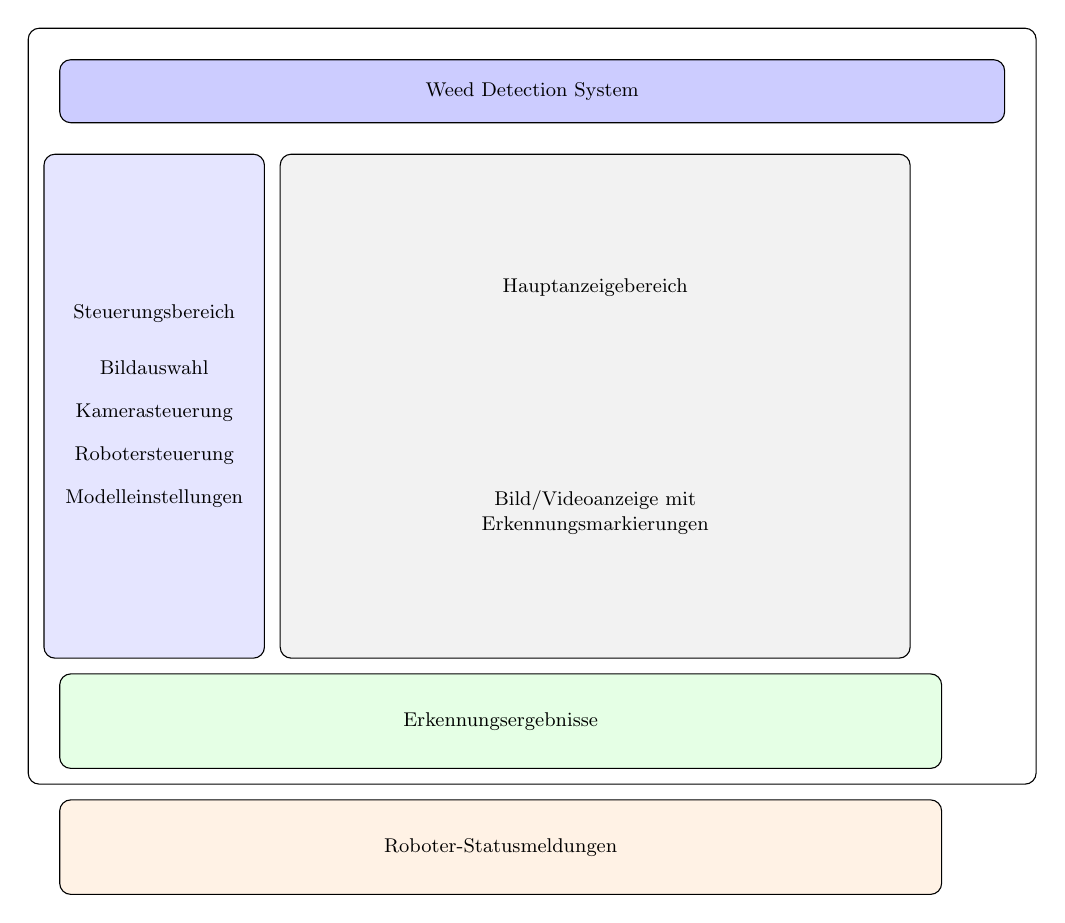
\begin{tikzpicture}[
        scale=0.8,
        transform shape,
        every node/.style={draw, rounded corners},
        section/.style={rectangle, minimum width=3cm, minimum height=1.5cm, align=center, font=\small}
    ]
    
    % Äußerer Rahmen für das gesamte Fenster
    \node[draw, rectangle, minimum width=16cm, minimum height=12cm, align=center] (window) {};
    
    % Titel
    \node[section, fill=blue!20, minimum width=15cm, minimum height=1cm, align=center] (title) at (0, 5) {Weed Detection System};
    
    % Linke Steuerungsleiste
    \node[section, fill=blue!10, minimum width=3.5cm, minimum height=8cm, align=center] (controls) at (-6, 0) {Steuerungsbereich\\[0.5cm]Bildauswahl\\[0.3cm]Kamerasteuerung\\[0.3cm]Robotersteuerung\\[0.3cm]Modelleinstellungen};
    
    % Hauptbildbereich
    \node[section, fill=gray!10, minimum width=10cm, minimum height=8cm, align=center] (main_display) at (1, 0) {Hauptanzeigebereich\\[3cm]Bild/Videoanzeige mit\\Erkennungsmarkierungen};
    
    % Ergebnisbereich unten
    \node[section, fill=green!10, minimum width=14cm, minimum height=1.5cm, align=center] (results) at (-0.5, -5) {Erkennungsergebnisse};
    
    % Roboter-Statusbereich unten
    \node[section, fill=orange!10, minimum width=14cm, minimum height=1.5cm, align=center] (robot_status) at (-0.5, -7) {Roboter-Statusmeldungen};
    
    \end{tikzpicture}
    \caption{Benutzeroberfläche des WeedDetector-Systems}
    \label{fig:user-interface}
\end{figure}

\subsection{Hauptfunktionen}
Die Benutzeroberfläche bietet folgende Hauptfunktionen:

\begin{enumerate}
    \item \textbf{Bildauswahl:} Ermöglicht das Laden eines Bildes aus dem Dateisystem zur Analyse.
    \item \textbf{Kamerasteuerung:} Aktiviert die Echtzeit-Bilderfassung über die angeschlossene Kamera.
    \item \textbf{Robotersteuerung:} Startet und stoppt die automatisierte Unkrauterkennung und -behandlung.
    \item \textbf{Empfindlichkeitseinstellung:} Ermöglicht die Anpassung des Konfidenzwertes für die Erkennung (0,05-0,95).
    \item \textbf{Erkennungsanzeige:} Zeigt erkannte Unkräuter mit Begrenzungsrahmen, Mittelpunktmarkierungen und Beschriftungen an.
    \item \textbf{Ergebnisprotokoll:} Listet detaillierte Informationen zu erkannten Objekten, einschließlich Koordinaten und Konfidenzwerten.
    \item \textbf{Roboter-Aktionsprotokoll:} Dokumentiert alle Aktionen und Statusmeldungen des Robotersystems.
\end{enumerate}

\section{Grundlegende Bedienung}

\subsection{Einzelbildanalyse}
Um ein einzelnes Bild auf Unkraut zu analysieren:
\begin{enumerate}
    \item Klicken Sie auf die Schaltfläche \textbf{"Select Image"}.
    \item Wählen Sie eine Bilddatei aus dem Dateiauswahldialog.
    \item Das System führt automatisch eine Erkennung durch und zeigt die Ergebnisse an.
    \item Passen Sie bei Bedarf den Konfidenzwert an, um die Erkennungsempfindlichkeit zu ändern.
\end{enumerate}

\subsection{Live-Kameraerkennung}
Für die Echtzeit-Unkrauterkennung mit der Kamera:
\begin{enumerate}
    \item Klicken Sie auf die Schaltfläche \textbf{"Start Camera"}.
    \item Die Kameraansicht wird im Hauptanzeigebereich angezeigt.
    \item Erkannte Unkräuter werden in Echtzeit markiert und im Ergebnisbereich aufgelistet.
    \item Zum Beenden der Kameraerkennung klicken Sie auf \textbf{"Stop Camera"}.
\end{enumerate}

\subsection{Robotersteuerung}
Zur Aktivierung des automatisierten Robotermodus:
\begin{enumerate}
    \item Stellen Sie sicher, dass die Kamera aktiviert ist oder aktivieren Sie sie.
    \item Klicken Sie auf die Schaltfläche \textbf{"Start Robot"}.
    \item Der Roboter beginnt mit der automatischen Unkrauterkennung und -behandlung.
    \item Alle Roboterhandlungen werden im Roboter-Statusbereich protokolliert.
    \item Bei Erkennung von Unkraut stoppt der Roboter automatisch für eine genauere Analyse.
    \item Zum manuellen Stoppen des Roboters klicken Sie auf \textbf{"Stop Robot"}.
\end{enumerate}

\section{Erweiterte Funktionen}

\subsection{Anpassung der Erkennungsparameter}
Die Erkennungsgenauigkeit kann durch Anpassung des Konfidenzwertes optimiert werden:
\begin{itemize}
    \item \textbf{Niedriger Konfidenzwert (0,05-0,25):} Erkennt mehr potenzielle Unkräuter, kann aber zu falschen Erkennungen führen.
    \item \textbf{Mittlerer Konfidenzwert (0,25-0,50):} Bietet eine ausgewogene Erkennungsrate für die meisten Anwendungen.
    \item \textbf{Hoher Konfidenzwert (0,50-0,95):} Reduziert Falscherkennungen, kann aber auch tatsächliche Unkräuter übersehen.
\end{itemize}

\subsection{Interpretation der Erkennungsergebnisse}
Die Erkennungsergebnisse werden in folgenden Formaten dargestellt:
\begin{itemize}
    \item \textbf{Visuelle Markierungen:}
    \begin{itemize}
        \item Rote Begrenzungsrahmen um erkannte Unkräuter
        \item Grüne Kreuze an den Mittelpunkten der erkannten Objekte
        \item Textbeschriftungen mit Klasse, Koordinaten und Konfidenzwert
    \end{itemize}
    \item \textbf{Textbasierte Ausgabe:}
    \begin{itemize}
        \item Nummerierte Liste erkannter Objekte
        \item Klassenname jedes erkannten Objekts
        \item X/Y-Koordinaten des Mittelpunkts
        \item Konfidenzwert der Erkennung
    \end{itemize}
\end{itemize}

\chapter{Modelltraining und -anpassung}

\section{Vorbereitung des Trainingsdatensatzes}
Die Qualität des Erkennungsmodells hängt maßgeblich von der Qualität und Vielfalt des Trainingsdatensatzes ab.

\subsection{Datenannotation}
Die Annotation der Trainingsdaten kann mit folgenden Tools durchgeführt werden:
\begin{itemize}
    \item \textbf{Roboflow:} Online-Plattform mit intuitiver Benutzeroberfläche
    \item \textbf{LabelImg:} Lokales Open-Source-Tool für YOLO-Annotationen
    \item \textbf{CVAT:} Leistungsstarkes webbasiertes Annotationstool
\end{itemize}

\subsection{Datenaugmentierung}
Zur Verbesserung der Modellrobustheit werden folgende Augmentierungstechniken empfohlen:
\begin{itemize}
    \item Horizontale und vertikale Spiegelung
    \item Rotation (±15° bis ±90°)
    \item Zufällige Zuschnitte (0-20\%)
    \item Helligkeits- und Kontrastvariationen (±10-20\%)
    \item Sättigungsanpassungen (±20\%)
\end{itemize}

\section{Durchführung des Trainings}
Der Trainingsprozess kann sowohl lokal als auch in der Cloud durchgeführt werden.

\subsection{Training starten}
Starten Sie das Training mit dem folgenden Befehl:
\begin{lstlisting}[language=bash]
python train.py --data data/data.yaml --epochs 50 --img 640 --batch 16
\end{lstlisting}

Trainingsparameter können je nach verfügbarer Hardware angepasst werden:
\begin{itemize}
    \item \texttt{--epochs}: Anzahl der Trainingsdurchläufe (empfohlen: 50-300)
    \item \texttt{--img}: Bildgröße für das Training (empfohlen: 640)
    \item \texttt{--batch}: Batch-Größe (an verfügbaren GPU-Speicher anpassen)
\end{itemize}

\section{Modellbewertung und -optimierung}
Nach Abschluss des Trainings sollte das Modell bewertet und optimiert werden.

\subsection{Bewertungsmetriken}
Die wichtigsten Metriken zur Bewertung des Modells sind:
\begin{itemize}
    \item \textbf{mAP (mean Average Precision):} Gesamtgenauigkeit über alle Klassen
    \item \textbf{Precision:} Verhältnis korrekter Erkennungen zu allen Erkennungen
    \item \textbf{Recall:} Verhältnis korrekter Erkennungen zu allen tatsächlichen Objekten
    \item \textbf{F1-Score:} Harmonisches Mittel aus Precision und Recall
\end{itemize}

\subsection{Feinabstimmung des Modells}
Bei unzureichender Leistung können folgende Optimierungsschritte durchgeführt werden:
\begin{enumerate}
    \item \textbf{Daten verbessern:} Mehr Trainingsbilder, bessere Annotation, zusätzliche Augmentierung
    \item \textbf{Hyperparameter anpassen:} Lernrate, Epochenzahl, Batch-Größe
    \item \textbf{Modellarchitektur ändern:} Größeres/kleineres Basismodell (YOLOv8n, YOLOv8s, YOLOv8m, YOLOv8l, YOLOv8x)
    \item \textbf{Transfer Learning:} Training auf vortrainiertem Modell für verwandte Domänen
\end{enumerate}

\section{Fehlerbehandlung und Logging}
Das System implementiert eine umfassende Fehlerbehandlung, um Robustheit zu gewährleisten:

\begin{itemize}
    \item \textbf{Exception Handling:} Alle kritischen Operationen sind mit spezifischen Exception-Handlern umgeben.
    \item \textbf{Fehlerprotokolle:} Fehler werden sowohl in der Konsole als auch in der GUI angezeigt.
    \item \textbf{Fallback-Mechanismen:} Bei Problemen mit benutzerdefinierten Modellen erfolgt ein Fallback auf das Standardmodell.
    \item \textbf{Robuste Kameraintegration:} Sichere Behandlung von Kamerazugriffsfehlern und Bildverarbeitungsproblemen.
\end{itemize}

\chapter{Wartung und Weiterentwicklung}

\section{Bekannte Einschränkungen}
Das aktuelle System hat folgende bekannte Einschränkungen:

\begin{itemize}
    \item \textbf{Rechenleistung:} Die Echtzeiterkennung benötigt ausreichende CPU/GPU-Ressourcen.
    \item \textbf{Lichtempfindlichkeit:} Die Erkennungsgenauigkeit variiert je nach Lichtverhältnissen.
    \item \textbf{Modellspezifität:} Das Modell funktioniert am besten für die Unkrautarten, auf die es trainiert wurde.
    \item \textbf{GUI-Beschränkungen:} Die Tkinter-Oberfläche hat eingeschränkte Anpassungsmöglichkeiten.
\end{itemize}

\section{Erweiterungsmöglichkeiten}
Folgende Erweiterungen sind für zukünftige Versionen geplant:

\begin{enumerate}
    \item \textbf{Erweiterte Roboterintegration:} Unterstützung für komplexere Roboterhardware und -steuerung.
    \item \textbf{Cloud-Integration:} Anbindung an Cloud-Dienste für Modelltraining und Datenspeicherung.
    \item \textbf{Mehrsprachige Unterstützung:} Internationalisierung der Benutzeroberfläche.
    \item \textbf{Mobile App:} Entwicklung einer begleitenden mobilen Anwendung für Felddiagnosen.
    \item \textbf{Kartenintegration:} Geo-Tagging und Kartierung erkannter Unkrautbereiche.
    \item \textbf{Verbesserte Bildvorverarbeitung:} Automatische Bildkorrektur für verschiedene Lichtverhältnisse.
\end{enumerate}

\section{Wartungsrichtlinien}
Zur langfristigen Wartung der Anwendung sollten folgende Richtlinien beachtet werden:

\begin{itemize}
    \item \textbf{Regelmäßige Updates:} Aktualisierung der Abhängigkeiten, insbesondere von OpenCV und YOLOv8.
    \item \textbf{Modellneuevaluierung:} Periodische Neubewertung und ggf. Neutraining des Erkennungsmodells.
    \item \textbf{Codeüberprüfung:} Regelmäßige statische Codeanalyse mit Bandit, Snyk und Pylint.
    \item \textbf{Dokumentationsaktualisierung:} Aktualisierung der Dokumentation bei Änderungen am Code oder an Funktionen.
    \item \textbf{Testabdeckung:} Aufrechterhaltung und Erweiterung der automatisierten Testabdeckung.
\end{itemize}

\chapter{Fazit und Ausblick}

\section{Projektergebnisse}
Der WeedDetector repräsentiert eine erfolgreiche Integration moderner Computer-Vision-Technologien in landwirtschaftliche Anwendungen. Das System bietet:

\begin{itemize}
    \item Eine benutzerfreundliche Oberfläche für die Unkrauterkennung
    \item Ein anpassbares und erweiterbares YOLO-basiertes Erkennungsmodell
    \item Eine modulare, wartbare Architektur nach dem MVC-Muster
    \item Eine vollständige Containerisierung für einfache Bereitstellung
\end{itemize}

\section{Zukünftige Forschungsrichtungen}
Basierend auf den Erfahrungen aus diesem Projekt ergeben sich folgende zukünftige Forschungs- und Entwicklungsrichtungen:

\begin{enumerate}
    \item \textbf{Multi-Spektralanalyse:} Integration von Infrarot- und Multispektraldaten für verbesserte Erkennung.
    \item \textbf{Drohnenintegration:} Anpassung des Systems für den Einsatz auf landwirtschaftlichen Drohnen.
    \item \textbf{Federated Learning:} Verteiltes Modelltraining zwischen verschiedenen landwirtschaftlichen Betrieben.
    \item \textbf{Präzisionssprühmechanismen:} Entwicklung präziser Mechanismen zur gezielten Behandlung einzelner Unkrautpflanzen.
    \item \textbf{Langzeitüberwachung:} Systeme zur kontinuierlichen Überwachung und Analyse der Unkrautentwicklung über Wachstumsperioden hinweg.
\end{enumerate}

\section{Abschließende Bewertung}
Der WeedDetector stellt einen bedeutenden Schritt in Richtung nachhaltiger, präziser Landwirtschaft dar. Die entwickelte Lösung bietet nicht nur praktische Vorteile für Landwirte, sondern trägt auch zu umweltfreundlicheren landwirtschaftlichen Praktiken bei.

Die modulare, erweiterbare Architektur des Systems ermöglicht zukünftige Anpassungen an spezifische landwirtschaftliche Anforderungen und die Integration neuer Technologien, sobald diese verfügbar werden.

\end{document}
